\documentclass[crop,tikz]{standalone}

\definecolor{presDark}{RGB}{39,1,136}
\definecolor{presDark2}{RGB}{87,80,149}
\definecolor{presLight}{RGB}{139,131,215}
\definecolor{presLight2}{RGB}{0,129,203}

\definecolor{presHighlight}{RGB}{215,50,50}


\begin{document}
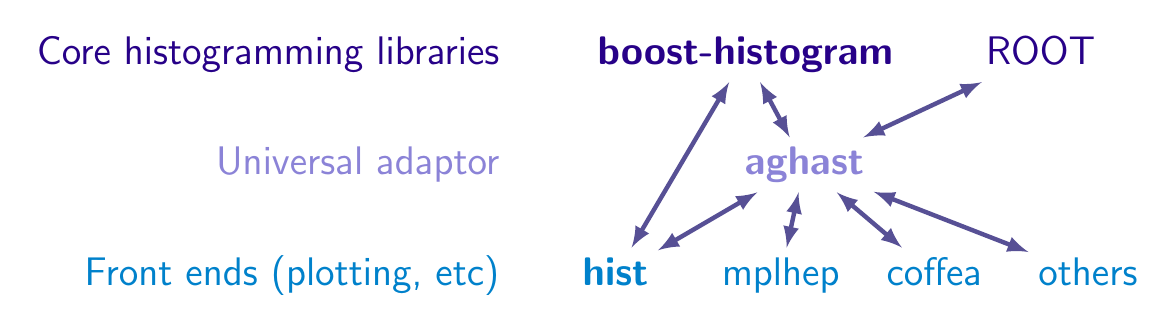
\begin{tikzpicture}[xscale=1.5, yscale=1.4, font=\sffamily\Large\vphantom{yH}]

\begin{scope}[presDark]
\node at (-2.5,0) [left] {Core histogramming libraries};
\node (bh) at (-.5,0)    {\textbf{boost-histogram}};
\node (root) at (2,0)    {ROOT};
\end{scope}

\begin{scope}[yshift=-1cm, presLight]
\node at (-2.5,0) [left] {Universal adaptor};
\node (aghast) at (0,0)  {\textbf{aghast}};
\end{scope}

\begin{scope}[yshift=-2cm, presLight2]
\node at (-2.5,0)     [left] {Front ends (plotting, etc)};
\node (hist) at (-1.6,0)     {\textbf{\textit{hist}}};
\node (mplhep) at (-.2,0)    {mplhep};
\node (physt) at (1.1,0)     {coffea};
\node (others) at (2.4,0)    {others};
\end{scope}

\begin{scope}[ultra thick, presDark2, latex-latex]
\draw (bh) -- (aghast);
\draw (root) -- (aghast);
\draw (mplhep) -- (aghast);
\draw (hist) -- (aghast);
\draw (hist) -- (bh);
\draw (physt) -- (aghast);
\draw (others) -- (aghast);
\end{scope}
\end{tikzpicture}
\end{document}
